\section{Polynomická funkce}

\begin{definition}\,
\begin{enumerate}[$i.$]
  \item Nechť $b \in \mathbb R$. Funkci $f:y = b$ nazveme \textbf{konstantní funkcí}.
  \item Nechť $a, b \in \mathbb R, a \neq 0$. Funkci $f:y= ax + b$ nazveme \textbf{lineární funkcí}.
\end{enumerate}
\end{definition}

\begin{figure}[ht!]
\begin{center}
  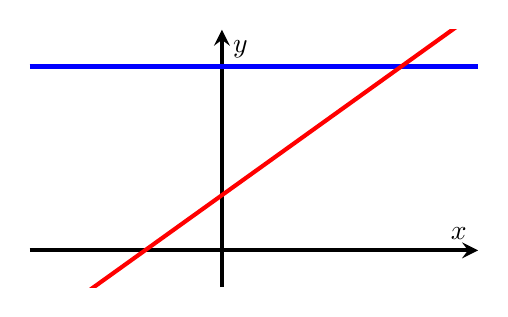
\begin{tikzpicture}
  \begin{axis}[
      axis lines = middle,
      xlabel = \(x\),
      ylabel = {\(y\)},
      xmin=-1.5,
      xmax=2,
      ymin=-0.2,
      ymax=1.2,
      xtick = \empty,
      ytick = \empty,
      line width=1.5pt,
      width=.6\textwidth,
      height=.4\textwidth,
  ]
  %Below the red parabola is defined
  \addplot [
      domain=-1.5:2,
      samples=500,
      color=blue,
  ]
  {1};

  \addplot [
      domain=-1.5:2,
      samples=500,
      color=red,
  ]
  {0.5*x+0.3};

  \end{axis}
  \end{tikzpicture}
  \caption{Graf konstantní (modře) a lineární (červeně) funkce}
\end{center}
\end{figure}

\begin{pozn}\,
  \begin{itemize}
    \item Definičním oborem konstantní i lineární funkce je $\mathbb R$. \\
          Oborem hodnot konstantní funkce je ${b}$.\\
          Oborem hodnot lineární funkce je $\mathbb R$.
    \item Grafem konstantní funkce je přímka rovnoběžná s osou $x$. \\
          Grafem lineární funkce je přímka, která není rovnoběžná s osou $x$ ani s osou $y$.
  \end{itemize}
\end{pozn}

\begin{veta}
  Nechť $f: y = ax + b, a \neq 0$ je lineární funkce. Pak platí:
  \begin{enumerate}[$i.$]
    \item $b=0 \implies f$ je lichá,\\
          $b \neq 0 \implies f$ není ani sudá, ani lichá;
    \item $a > 0 \implies f$ je rostoucí,\\
          $a < 0 \implies f$ je klesající;
    \item $f$ není ani shora, ani zdola omezená;
    \item $f$ nemá extrémy;
    \item $f$ není periodická.
  \end{enumerate}
\end{veta}

\begin{proof}\,
  \begin{enumerate}[$i.$]
    \item $b=0 \implies f:y= ax = f(x) \land -ax = -f(x) \implies f$ je lichá\\
          $b\neq 0 \implies f:y = ax + b = f(x) = -ax + b \implies f$ není sudá ani lichá
    \item $a>0 \implies x_1 < x_2 \implies ax_1 < ax_2 \implies ax_1 + b < ax_2 + b \implies f$ je rostoucí\\
          $a<0 \implies x_1 < x_2 \implies ax_1 > ax_2 \implies ax_1 + b > ax_2 + b \implies f$ je klesající
    \item Obor hodnot je $\mathbb R \implies f$ není omezená.
    \item Plyne z grafu.
    \item Plyne z grafu nebo z toho, že $f$ je ryze monotónní. \qedhere
  \end{enumerate}
\end{proof}

\begin{definition}
  Nechť $a,b,c \in \mathbb R, a \neq 0$. Pak funkci $f:y = ax^2 + bx+ c$ nazýváme \textbf{kvadratickou funkcí}.
\end{definition}

\begin{figure}[ht!]
  \centering
  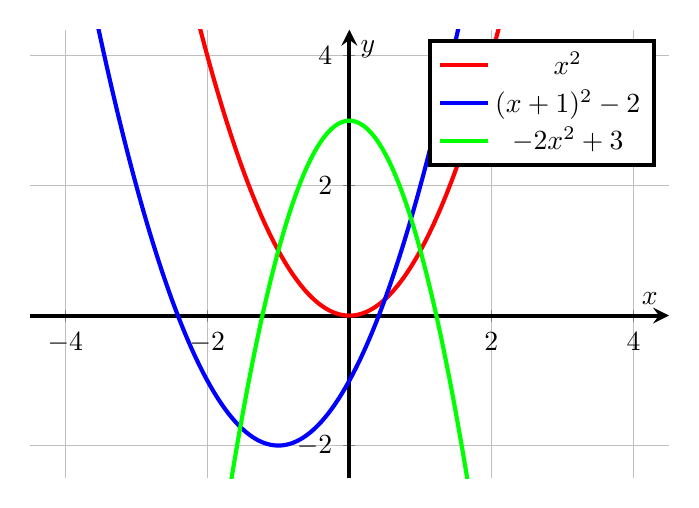
\begin{tikzpicture}
    \begin{axis}[
        axis lines = middle,
        xlabel = \(x\),
        ylabel = {\(y\)},
        line width=1.5pt,
        width=.8\textwidth,
        height=.6\textwidth,
        ymin=-2.5,
        ymax=4.4,
        xmin=-4.5,
        xmax=4.5,
        grid
    ]
    %Below the red parabola is defined
    \addplot [
        domain=-4:4,
        samples=500,
        color=red,
    ]
    {x^2};
    \addlegendentry{\(x^2\)}

    \addplot [
        domain=-4:4,
        samples=500,
        color=blue,
        ]
        {(x+1)^2-2};
    \addlegendentry{\((x+1)^2-2\)}

    \addplot [
        domain=-4:4,
        samples=500,
        color=green,
        ]
        {-2*x^2+3};
    \addlegendentry{\(-2x^2+3\)}

    \end{axis}
    \end{tikzpicture}
  \caption{Grafy různých kvadratických funkcí}
\end{figure}

\begin{pozn}\,
  \begin{itemize}
    \item Definičním oborem kvadratické funkce je $\mathbb R$.
    \item Grafem kvadratické funkce je parabola.
  \end{itemize}
\end{pozn}

\begin{veta}
  Nechť $f:y = ax^2, a \neq 0$ je kvadratická funkce. Pak platí:
  \begin{center}
    \begin{tabularx}{\textwidth}{ l | l  l }
        \, & $a>0$ & $a<0$ \\
        \hline
        obor hodnot & $H(f) = \mathbb R^{+}_0$ & $H(f) = \mathbb R^{-}_0$ \\
        parita & sudá & sudá \\
        monotónnost & $x \in (-\infty, 0\rangle$ -- klesající & $x \in (-\infty, 0\rangle$ -- rostoucí \\
        \, & $x \in \langle 0, \infty)$ -- rostoucí & $x \in \langle 0, \infty)$ -- klesající \\
        omezenost & zdola omezená & zdola neomezená \\
        \, & shora neomezená & shora omezená \\
        extrémy &  ostré minimum v bodě $x_0=0$ & ostré maximum v bodě $x_0=0$ \\
        periodicita & neperiodická & neperiodická
    \end{tabularx}
  \end{center}
\end{veta}

\begin{proof}
    Dokážeme jen paritu a monotonii. Ostatní plyne z grafu.
    \begin{enumerate}
        \item[$i.$] parita: $D(f) = \mathbb R$ -- platí, $f(-x)=a(-x)^2=ax^2=f(x) \implies f$ je sudá
        \item[$ii.$] monotonie: \begin{itemize}
        \item $a>0 \land x\in \left (-\infty,0\right >$: \\
        Je-li $x_1<x_2$, pak $ax_1^2 > ax_2^2 \iff ax_1 <ax_2 \iff ax_1^2>ax_1x_2 \land ax_1x_2 > ax_2^2 \implies$ platí.
            \item $a>0 \land x\in \left <0,\infty\right )$: \\
            Je-li $x_1<x_2$, pak $ax_1^2 > ax_2^2 \iff ax_1 <ax_2 \iff ax_1^2>ax_1x_2 \land ax_1x_2 > ax_2^2 \implies$ platí.\qedhere
        \end{itemize}
    \end{enumerate}
\end{proof}

\begin{veta}
  Nechť $f:y = ax^2+bx+c, a \neq 0$ je kvadratická funkce. Pak platí:
  \begin{center}
    \begin{tabularx}{\textwidth}{ l | l  l }
        \, & $a>0$ & $a<0$ \\
        \hline
        obor hodnot & $H(f) = \left <c-\frac{b^2}{4a}, \infty \right)$ & $H(f) = \left (-\infty, c-\frac{b^2}{4a}\right >$ \\
        parita & obecně není ani sudá, ani lichá & \, \\
        monotónnost & $x \in \left (-\infty, -\frac{b}{2a} \right >$ -- klesající & $x \in \left (-\infty, -\frac{b}{2a} \right >$ -- rostoucí \\
        \, & $x \in \left < -\frac{b}{2a}, \infty \right )$ -- rostoucí & $x \in \left < -\frac{b}{2a}, \infty \right )$ -- klesající \\
        omezenost & zdola omezená & zdola neomezená \\
        \, & shora neomezená & shora omezená \\
        extrémy &  ostré minimum v bodě $x_0=-\frac{b}{2a}$ & ostré maximum v bodě $x_0=-\frac{b}{2a}$ \\
        periodicita & neperiodická & neperiodická
    \end{tabularx}
  \end{center}
\end{veta}

\begin{definition}
    Nechť $P(x)\in \mathbb R[x]$ je polynom. Pak funkci $f:y=P(x)$ nazveme \textbf{polynomickou funkcí}.
\end{definition}

\begin{figure}[ht!]
  \centering
  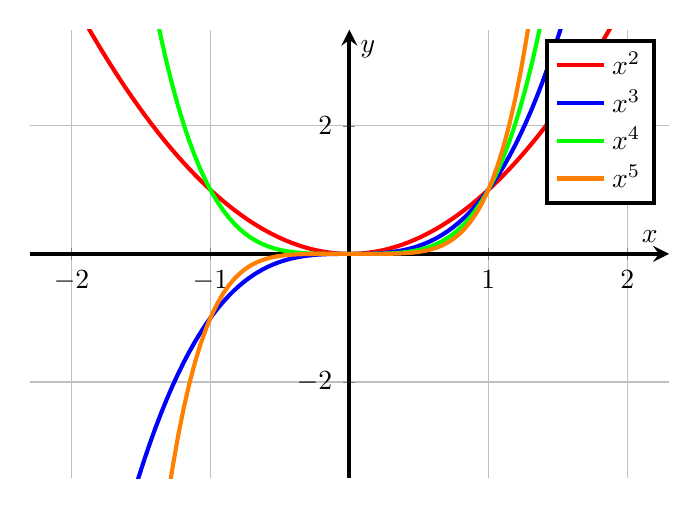
\begin{tikzpicture}
    \begin{axis}[
        axis lines = middle,
        xlabel = \(x\),
        ylabel = {\(y\)},
        line width=1.5pt,
        width=.8\textwidth,
        height=.6\textwidth,
        ymin=-3.5,
        ymax=3.5,
        xmin=-2.3,
        xmax=2.3,
        grid
    ]
    %Below the red parabola is defined
    \addplot [
        domain=-2:2,
        samples=100,
        color=red,
    ]
    {x^2};
    \addlegendentry{\(x^2\)}

    \addplot [
        domain=-2:2,
        samples=100,
        color=blue,
        ]
        {x^3};
    \addlegendentry{\(x^3\)}

    \addplot [
        domain=-2:2,
        samples=100,
        color=green,
        ]
        {x^4};
    \addlegendentry{\(x^4\)}

    \addplot [
        domain=-2:2,
        samples=100,
        color=orange,
        ]
        {x^5};
    \addlegendentry{\(x^5\)}

    \end{axis}
    \end{tikzpicture}
  \caption{Grafy funkcí tvaru $x^n$}
\end{figure}

\begin{pozn}\,
    \begin{enumerate}[$i.$]
        \item Definičním oborem polynomické funkce je $\mathbb R.$
        \item Jestliže je stupeň polynomu lichý, pak je obor hodnot $\mathbb R.$ Jestliže je sudý a $a_n > 0,$ je obor hodnot interval $\left <c,\infty \right )$,
        v opačném případě je to interval $\left (-\infty, c\right >$, kde $c \in \mathbb R$.
    \end{enumerate}
\end{pozn}

\begin{definition}
    Nechť $y=f(x)$ je polynomická funkce. Pak $c\in \mathbb R$ nazveme \textbf{nulovým bodem} polynomické funkce $f$ právě tehdy, když $f(c)=0.$
\end{definition}

\begin{pozn}
    Nulovým bodem polynomické funkce rozumíme kořen polynomu.
\end{pozn}
